\section{Part by Part information}
In this document some locations are indicated with front, back, left, and right. These are seen as standing behind the bicycle and looking from rear wheel to front wheel. (Or from electronic box to handlebar.)

%===============[ Mechatronic Physical things ]
\subsection{Mechatronic/Physical Things}
\begin{figure}
    \centering
    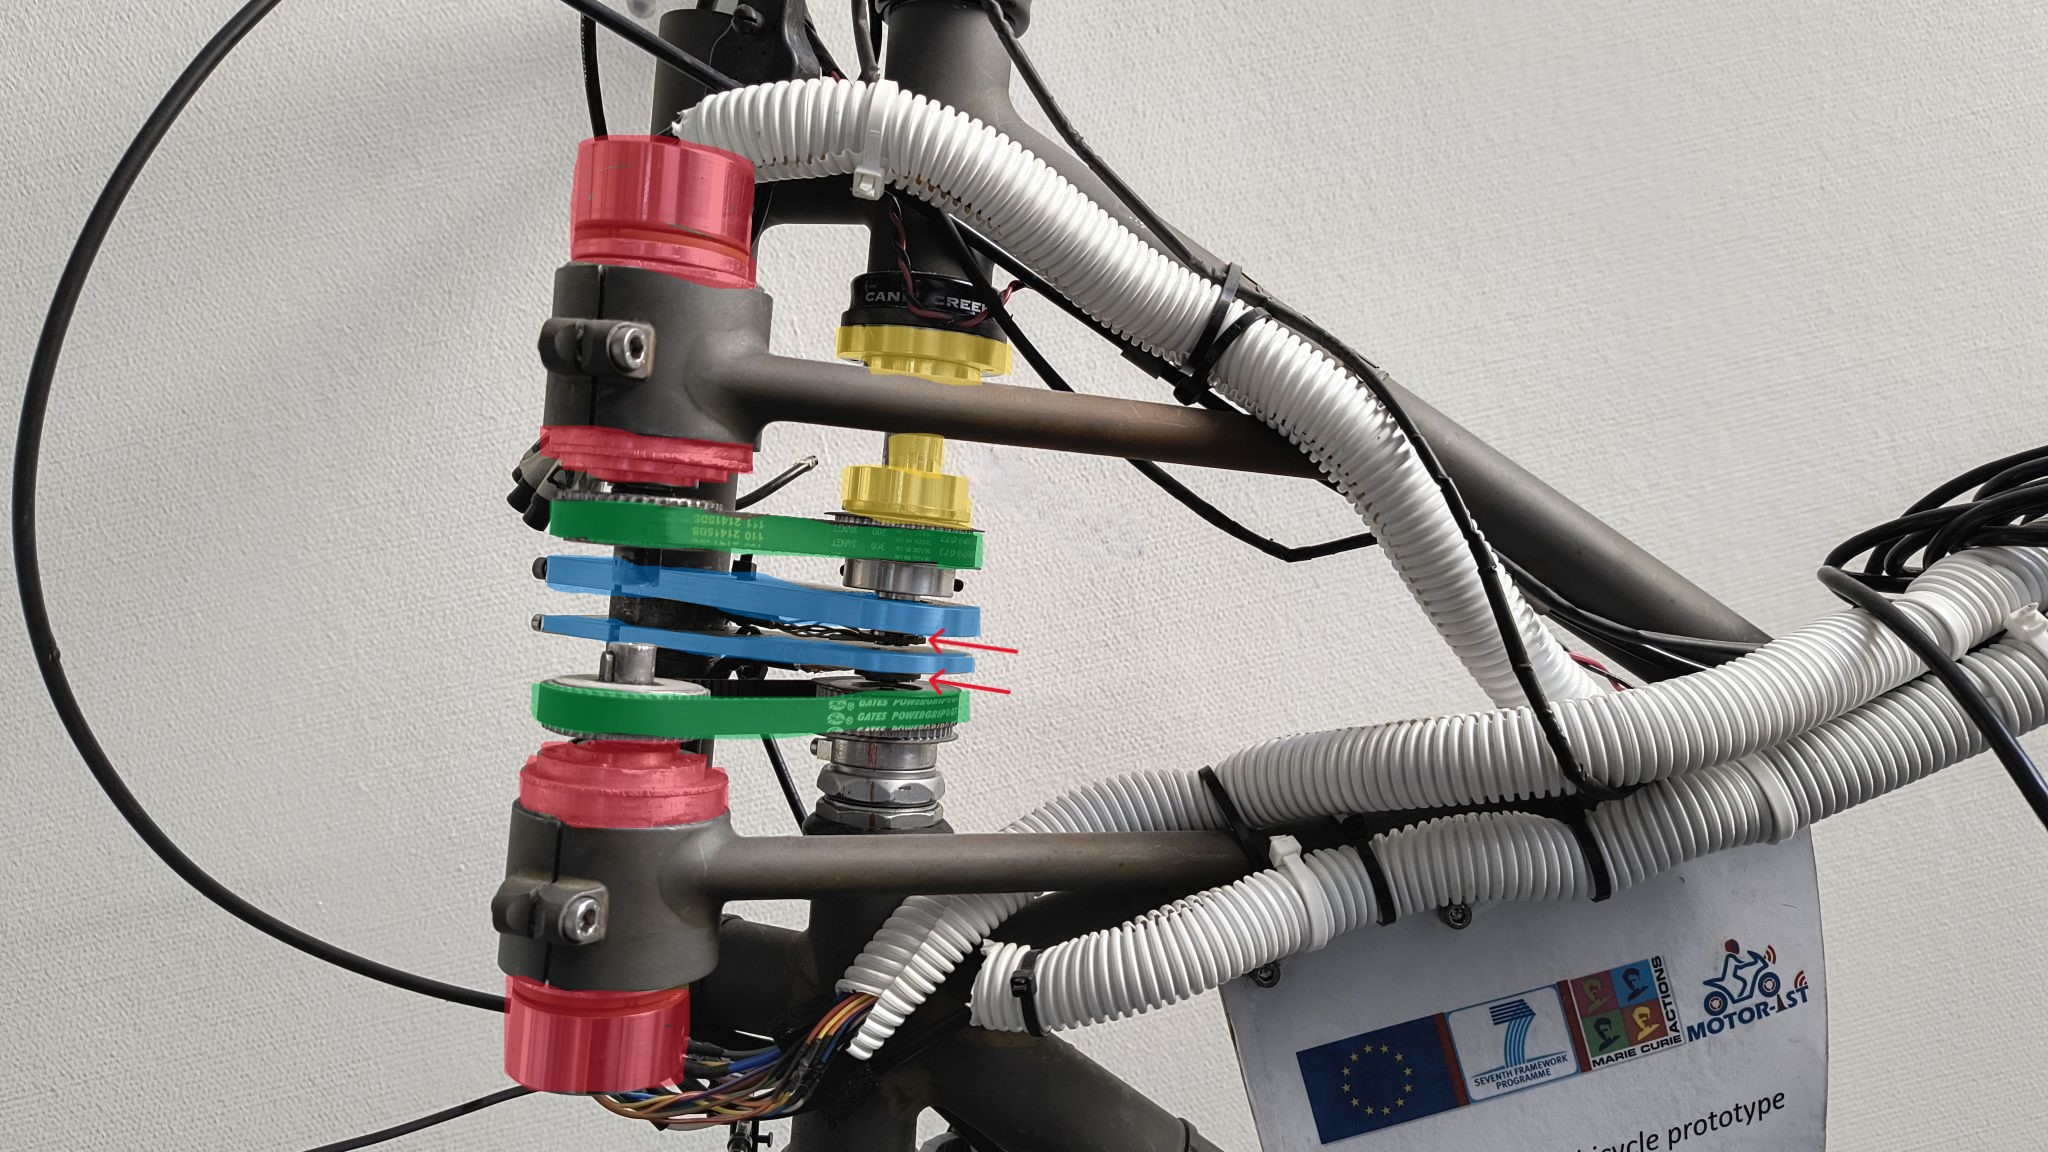
\includegraphics[width=\textwidth]{Img/highlight_locations.jpg}
    \caption{Location of multiple parts in the steer-by-wire steering system. Here the (broken) steer torque sensor is highlighted in yellow, the belt drives in green, the motors in red, and the absolute encoder fixtures in blue. The red arrows indicate the location of the absolute encoders}
    \label{fig:location_highlights}
\end{figure}

\subsubsection{DC motors}
The motors in the drive train consists out of two Maxon EC45 brushless DC motors.
These motors are controlled by motor drivers.
They are indicated in red in \autoref{fig:location_highlights}

\subsubsection{Transmission between the Motors and Handlebar/Fork}
The motors are connected to the steer and front fork through two respective transmissions both consisting of a Maxon GP42C planetary gearhead (36:1 reduction ratio), and a belt drive (1:1 reduction ratio). The belt drive is indicated in green in \autoref{fig:location_highlights}

\subsubsection{Electric Propulsion System}
The steer-by-wire (sbw) bicycle is an e-bike. 
A motor (magic pie 5) in the hub of the rear wheel actuates the wheel.
The wheel is controlled by the throttle on the right part of the handlebar, and is able to use cruise control.
See the section `2.2 Rear Wheel' in the documentation of Simonas.

\subsubsection{Electric Brakes}
The brakes are electric.
In other words, a sensor measures if the brakes are activated.
These sensors are connected to the front and back brakes through two of the cables labelled A to D that are near the head tube.

\subsubsection{Battery}
A large battery is attached to the seat tube.
The make, model, voltage, and ampere hour are unknown.
By pressing the button on the battery, LEDs will light up indicating the the charge state of the battery.

The battery has a charger that fits on the small white connector at the top of the battery.
The charger to this battery is inside a brown cardboard box labeled `steer-by-wire charger'. 

\subsubsection{Counter Weight}
The bicycle with SIL controller was driving at a speed such that it was self stabilising.
Without any external inputs the bicycles heading rate was a nonzero value with a constant sign. 
In other words it drifted towards the side.
During the early experiments, the drift consistently went to one side.
To try and counteract this drift, a weight of 0.975kg was placed under the saddle (the original force transducer location) at the opposite side of the drift. 
The source of the drift still remains unknown.
Currently the weight is removed.

\subsubsection{Lashing Straps}
The experiment for model matching was conducted only using the fork motor. 
The steer is not used. 
Therefore the steer was fastened to the frame (left and right handlebar to sadle post), using lashing straps.

\subsubsection{Metal Connection Rod}
The sbw steering system uses a metal rod as a fail save in the case the bike loses power while someone is riding on it. 
This rod connects the front wheel to the handlebar. 
It has some play to allow undisturbed steering when there are no issues. 
The wing nuts can be adjusted to increase or decrease this free movement range.



%===============[ Sensors ]
\subsection{Sensors}
\subsubsection{Motor Encoders}
The motor driver uses two absolute angular encoders (RMB20SC 13 bit) to sense the angular position of the motors.
These encoders are directly connected with the motor controllers.
They are located at the red arrows in \autoref{fig:location_highlights}.

The encoders are mounted to the bicycle by the fixtures highlighted in blue.
Due to the unfortunate design of the lower fixture, it difficult to properly install the fork encoder, making the read out inacurate.
See \autoref{sec:fork_encoder} for more detail.

\subsubsection{Force Transducer}
A 100kg Force Transducer was originally attached to the saddle post to measure pulling forces. 
Currently it is placed back to this location.
I made an add-on piece that fits on the left steering handle (should be in the sbw storage box).
This piece allows the force transducer to be fastened to the steer, and function as a steer force sensor.
The rubber cover of the handlebar needs to be taken of first, then the add-on piece can be wedged on the steer. 
The force transducer can then be mounted on the add-on piece with a M12 bolt and nut.

I could not find the make and model, but calibration showed a linear relation between signal and applied force.
The results of the calibration can be found in the 'global variables > constants' section at the start of the \href{https://github.com/mechmotum/sbw_bicycle_with_model_matching/tree/master/teensy/src}{teensy/src/main.cpp} file.

\subsubsection{Speed an Cadence Encoder}
The swb bike has two relative encoders (GTS35/GTS45 gear tooth sensor) and encoder disks, which are used to measure the speed and the cadence.
These sensors are placed at the rear wheel center, and at the pedals.
These sensors have a built-in attachment part that allows for a nut and bolt to fasten the sensor to an external part. 
For the original speed sensor, this built-in attachment broke off. 
This sensor is now taped to the luggage carrier and labeled ENCODER. 
To still measure the bicycle speed, the encoder that measures the cadence was dismantled and used instead. 

Additionally an add on piece was made from wood, because the original fixation was wrongly orientated.
This caused the sensor to not be able to differentiate direction. 
This add-on piece allows the sensor to be rotated with 90 degrees, thereby correctly assembling the sensor $\longleftrightarrow$ encoder disk set-up.

The sensor itself needs to be calibrated again. The speeds indicated by the sensor and the speed indicated by the treadmill do not match. 
See my thesis (Model Matching Control Applied to Bicycles) for further information.

The speed encoder placed at the rear wheel is connected to the microcontroller extension board. % at J5.
This is however not a direct connection, as there is a small circuit soldered between the encoder and the cable connecting it to the PCB. 
(It is taped of with the black and yellow tape.) 
This is a signal termination circuit, as recommended the manufacturers. 
See the 'GTS35/GTS45 gear tooth sensor' documentation on page 5.

\subsubsection{Torque Sensor in the Steering Column} \label{sec:steer_torque_sensor}
The steer had a torque sensor located in the steering column, see the yellow highlight in \autoref{fig:location_highlights}.
The torque sensor is designed by Christos Christoforidis in his thesis "The effect of haptic feedback in the balance task of bicycling". 
It makes use of multiple strain gauge sensors. 
These gauge sensors were broken upon investigation, so I removed them from the metal part. 
The wires lead to the prototyping board attached on the left wall of the electronics box. 
I removed these wires as well, as they were a cause for noise interference on other sensors.
Thus the gauge sensors are completely removed from the bicycle, and this torque sensor is currently OUT OF USE. 

It is possible to use the \href{https://www.kistler.com/US/en/p/reaction-torque-transducer-9349a/000000000018007698}{Kistler torque sensor} and its accompanying \href{https://www.kistler.com/US/en/cp/industrial-miniature-charge-amplifiers-miniamp-5030a/P0000265}{Kistler mini opAmp}. 
The manual can be found in PDF form on the surfdrive or physically in the sbw storage box.
Both objects are currently installed on the bicycle simulator in the basement.
Although technically they can be disassembled and re-assembled into the sbw bike. 
This equipment is very delicate, so be absolutely certain you want to use these and not a cheaper/simpler variant.

\subsubsection{IMU}
The electronics box contains a seperate IMU break out board (\href{https://learn.sparkfun.com/tutorials/mpu-9250-hookup-guide/all}{sparkfun MPU 9250}).
Here is a link to to the \href{https://cdn.sparkfun.com/datasheets/Sensors/IMU/SparkFun_MPU-9250_Breakout.pdf}{break out board's schematics}.
I needed to install a separate IMU as I could not get the IMU chip on the microcontroller extension board to be detected by the microcontroller. I was able to detect and use the IMU chip when connecting a spare teensy to a spare microcontroller extension PCB. My guess is that either the IMU chip on the installed extension PCB is broken, or the other electronics connected to the PCB and microcontroller prevent the IMU chip from being detected via the SPI protocol.

This IMU is mounted on the front wall and fortified with a wooden structure, such that the relative orientation of the bicycle and IMU remain constant.
The Teensy is \textit{directly} connected with the IMU through the \href{https://en.wikipedia.org/wiki/I%C2%B2C}{I2C} protocol.
I2C was chosen over SPI for two reasons.
First, I2C allowed for a higher read-out rate of the IMU data.
Secondly, for unknown reasons the teensy could not detect the IMU when using SPI. 
The teensy can detect the IMU breakout board if it is the only thing connected to the teensy, but not when teensy and IMU are integrated in the sbw's electronic circuit.

%===============[ PCB's and other electronic circuits
\subsection{PCB's and Other Electronic Circuits}
\subsubsection{Force Transducer Prototype Board}
Against the left wall there is a prototype board.
This board contains two \href{https://www.ti.com/lit/ds/symlink/ina125.pdf}{INA125} ICs, used to amplify the signal coming from Wheatstone bridge circuits.
One was used for the (now broken) steer torque sensor (see \autoref{sec:steer_torque_sensor}), the other is for the force transducer.
A constant supply voltage (of 10V) is regulated by a voltage regulator (\href{https://www.digikey.com/en/products/detail/stmicroelectronics/l7810cv/1038259}{L7810CV}) attached to the left wall of the electronic box. 
(See \autoref{fig:voltage_regulateor} for a picture of a voltage regulator.)
Lastly, the readout of the sensors via this circuit has some problems, as there is noise on the ground of the signal, see \autoref{sec:noise_on_ground} for more info.
\begin{figure}
    \centering
    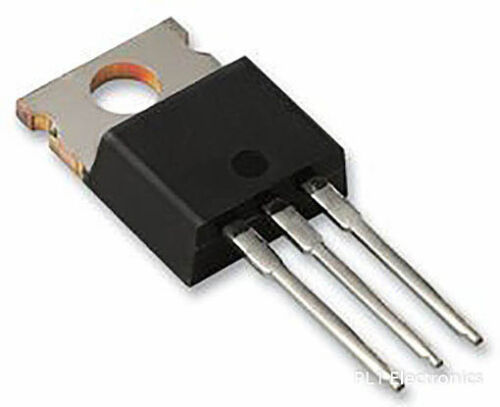
\includegraphics[width=0.2\textwidth]{Img/voltage_regulator.jpg}
    \caption{Picture of a voltage regulator}
    \label{fig:voltage_regulateor}
\end{figure}

\subsubsection{Power PCB}
One of the two large PCBs in the electronics box.
This PCB is designed to regulate the appropriate power to all the PCBs, sensors and ICs.
It houses the two motor drivers.
This board was designed by Oliver Lee, Georgios Dialynas, and Andrew Berry to be a general power distribution board for bicycles applied in both the bicycle simulator and the sbw bicycle. Therefore, not all functions on the PCB are used for the sbw operation.

The schematics of integrated circuits, and a 2D model (with layers) of the PCB can be found on either \href{https://github.com/oliverlee/gyropcb}{Oliver's Github repository} or its fork on \href{https://github.com/gdialynas/gyropcb}{Georgias's Github repository}.
These are the files \texttt{power\_pcb.brd} and \texttt{power\_pcb.sch} for the board and schematics respectively.
To read these two files, one needs download the program \textbf{Eagle} by Autodesk.
Although there is a premium software package, the \href{https://www.autodesk.com/products/eagle/free-download}{FREE version} is enough to view the board and schematic, see \href{https://learn.sparkfun.com/tutorials/how-to-install-and-setup-eagle/all}{a sparkfun blog} about the versatility of the free version.
You do need to make an account at autodesk for the software to work.

\subsubsection{Microcontroller Extension PCB} \label{sec:micro_extension_board}
The micro controller extension PCB is designed to extend the microcontrollers capabilities, and acts as an interface between the microcontroller and the rest of the electronics.
This board was designed by Oliver Lee, Georgios Dialynas, and Andrew Berry to be a general microcontroller extension board for bicycles applied in both the bicycle simulator and the sbw bicycle. Therefore, not all functions on the PCB are used for the sbw operation.

Originally the microcontroller would have been directly placed on the board in the two double row header pin slots labeled \texttt{EXT1} and \texttt{EXT2}.
However, the type of micro controller changed from an OLIMEX STM32-H405 to a \href{https://www.pjrc.com/teensy/}{Teensy} (currently teensy 4.1) that has a different pin configuration.
Therefore, the teensy is placed separate from the PCB.
Jumper wire connect the necessary pins between the teensy and the \texttt{EXT1} and \texttt{EXT2} header pins.
The \texttt{EXT1} or \texttt{EXT2} are labeled according to the old OLIMEX STM32-H405 controller pin numbering. (see \href{https://www.olimex.com/Products/ARM/ST/STM32-H405/resources/STM32-H405_UM.pdf}{page 9 of the manual}).

Some circuits on this PCB were broken/buggy, therefore the PCB was bug fixed post production.
What is done exactly and why both remain unknown to me, but I uncovered three instances.
The first instance of a bug is a missing MPU9250 chip (IMU).
There are supposed to be two IMU chips on the PCB.
One chip (at label \texttt{U10}) is connected to the \texttt{EXT1} pins, such that the microcontroller has direct access.
The other chip (at label \texttt{U13}) is an isolated circuit that can only be accessed trough the set of male pin headers (labelled \texttt{EXT3}) at the side of the board.
The first chip is \textit{not} soldered on the PCB.
To compensate for the missing IMU chip (\texttt{U10}), debug wires connect the \texttt{EXT1} pins to the second IMU chip (\texttt{U13}).

The second instance is the faulty motor driver read out circuit.
The motor drivers have an analog output signal that can give information on the motor (e.g. motor current).
Which information it gives can be programmed, see \autoref{sec:motor_drivers}.
The analog output given by the motor driver is between +4 V and -4 V.
The extension PCB has a circuit to transform the $\pm$4V to 0 till 3.3 V.
From what I understand, this circuit is broken.
If you want to read out the motor driver output, you have to remake the circuit externally, see  \autoref{sec:motor_driver_read_out}.

In the third instance, two chips are missing at location \texttt{U4} and \texttt{U5}.
These locations should have a \href{https://media.digikey.com/pdf/Data%20Sheets/Fairchild%20PDFs/74AC157,%2074ACT157.pdf}{74AC157 Quad 2-Input Multiplexer} chip.
Instead (with the use of some solder) the relative encoder signals are directly send to the teensy, and the absolute encoders are rerouted to somewhere else.
If you want to investigate further, look into the pcb design files via Eagle.

Again the schematics of integrated circuits, and a 2D model (with layers) of the PCB can be found on either \href{https://github.com/oliverlee/gyropcb}{Oliver's Github repository} or its fork on \href{https://github.com/gdialynas/gyropcb}{Georgias's Github repository}.
These are the files \texttt{mc\_pcb.brd} and \texttt{mc\_pcb.sch} for the board and schematics respectively, and also require Eagle to be viewed.

\subsubsection{Motor Drivers} \label{sec:motor_drivers}
The two motors in the steer-by-wire system each have their own \href{https://www.maxongroup.com/maxon/view/product/control/4-Q-Servokontroller/438725}{ESCON Module 50/5} motor driver, which are located on top of the power PCB.
The motor driver connected to \texttt{EXT1} and \texttt{EXT2} correspond to the handlebar motor, and \texttt{EXT3} and \texttt{EXT4} to the fork motor.
These motor drivers make sure the motor behaves according to the PWM commands of the microcontroller.
The motor drivers are \href{https://www.youtube.com/watch?v=-TC_ccQnk-Y&list=PLZXUEi3qPF8XuMxMWy3hmKjp807U61QaZ&index=6}{programmable}, and one can choose, among other things, the motor control mode, and what variables are represented on the output pins.
I am not 100\% certain, but currently the motor driver is programmed to have torque control, and the analog out 1 pin of the handlebar motor driver is set to portray the motor current.

It is not sure if the motor driver's 'motor current' output is the motor current send to the motor or the total current running through the motor.
From an experiment it is suggested it is the first.
In this experiment I rotated the steer, while not sending any torque commands to the motor. 
The measured current was zero for the entirety of the experiment.
Therefore, either the back EMF caused a current that is not measured, or the circuit is open when no commands are sent and no current can flow despite the back EMF.

\subsubsection{Motor Driver Analog OUT Transformer} \label{sec:motor_driver_read_out}
The ESCON Module 50/5 motor driver has two analog output pins.
Analog out 1 of the handlebar motor is programmed to show motor current and is connected to J10-2 of the power PCB.
I do not know what analog out 1 of the fork motor is programmed to, but it is connected to J11-2 of the power PCB
Analog out 2 is not connected to anything for both motor drivers.

The analog output is between -4V and +4V.
However, the teensy analog input pins go from 0V to 3.3V.
A circuit as shown by \autoref{fig:transformer_circuit} transform the motor driver voltage range to the teensy's voltage range, and filters possible noise.
This circuit is originally present on the extension PCB, but it is broken.
Therefore, to read out the motor driver's analog output you have to built this circuit yourself (on e.g. a breadboard), and install it between the power PCB and the teensy microcontroller. 
This is done by connecting J10-2 to the blue circle on the left, supplying the 3.3V by the teensy, connect all grounds to a common ground, and have one of the two orange circles on the right connected to an analog pin of the teensy.
Some explanation on how the circuit works can be found \href{https://electronics.stackexchange.com/questions/115502/convert-from-a-specifc-range-to-another-one#}{here} and \href{https://www.youtube.com/watch?v=mUbACZP-8Sw}{here}.
\begin{figure}
    \centering
    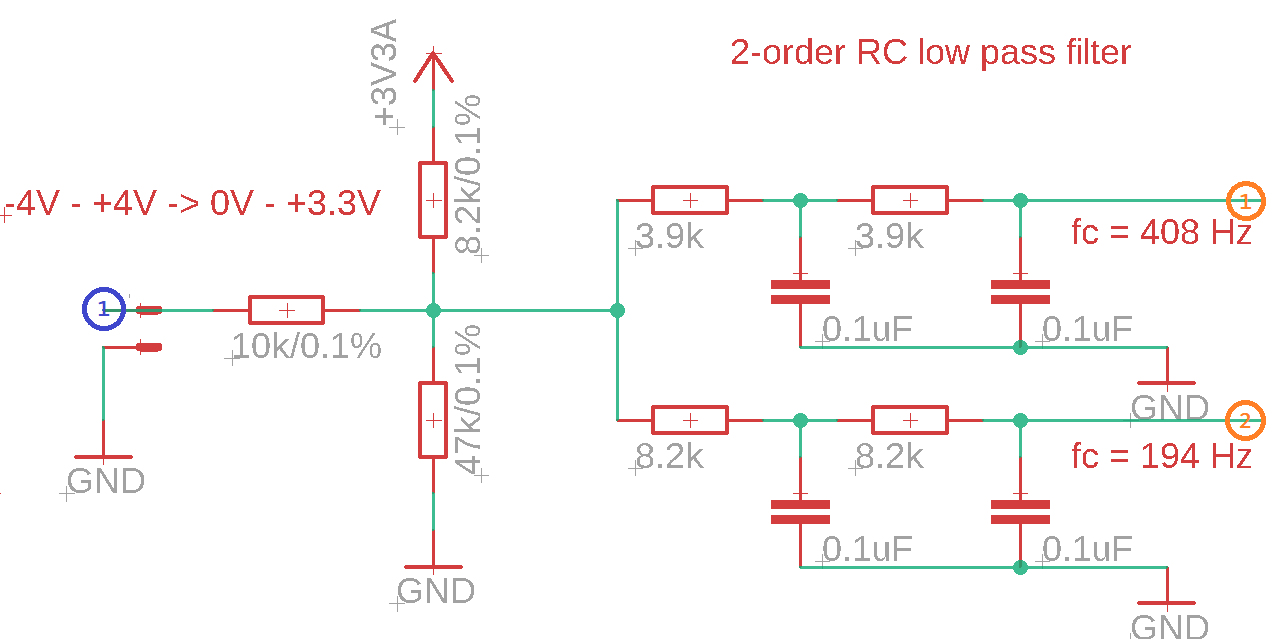
\includegraphics[width=\textwidth]{Img/motor_driver_to_teensy_voltage_transformer.PNG}
    \caption{Electrical circuit to read out the analog output of the motor driver. Taken from the schemetics of the microcontroller PCB designed by Oliver Lee, Georgios Dialynas, and Andrew Berry.}
    \label{fig:transformer_circuit}
\end{figure}



%===============[ Other
\subsection{Other}
\subsubsection{Switch}
On the same location as the propulsion throttle (right side of the steer) is a switch.
Currently this switch is not in use, as it was not required.
The code to read out the switch is commented out.
The switch was initially used to turn the MPC controller on or off in the experiments of Simonas.

\subsubsection{Handlebar LED}
There is an green LED on the handlebar that is controlled by the micro controller.
The LED is used as a status and error indicator.
The random loose hanging resistor on the left side of the box is part of the circuit belonging to the LED. (My guess is it is a pull up or pull down resistor.)

\subsubsection{Bluetooth}
Taped to the right side of the electronic box is a HC-05 bluetooth module.
These modules work in pairs, one being the main/sending module, the other being the sub/receiving module.
This means you need a second microcontroller and bluetooth module to communicate with the bluetooth module in the electronic box.
The role of the module (main or sub) needs to be programmed beforehand.
How to connect two modules to each other and how to program the HC-05 to be a sub or main can be found in these tutorials: 
\href{https://www.instructables.com/Arduino-Two-Way-Communication-Via-Bluetooth-HC-05/}{two way communication}, \href{https://www.youtube.com/watch?v=hyME1osgr7s}{example in video format}, \href{https://www.instructables.com/AT-command-mode-of-HC-05-Bluetooth-module/}{programming to be main/sub}.

Additionally you can link your phone to the one bluetooth module instead. In this way you only need one module.

Be aware: The data transmission over bluetooth is slow. So for applications where the communication needs to happen at high frequency, I would suggest another protocol.

\subsubsection{Micro Controller}
The microcontroller used is a \href{https://www.pjrc.com/store/teensy41.html}{Teensy 4.1}.
It is placed at the front of the electronics box.
The code on the teensy allows it to run in three modes.
A fully independent mode, where the teensy is powered by the battery and does not communicate with any external computer.
A semi independent mode, where the teensy is powered by the battery, but waits with executing the loop untill it has has wireless communication with an external computer.
And a dependent mode, where the teensy is powered by an external computer via USB, and also waits for communicates with that computer via the USB before running the loop.

When the teensy is powered by the battery, it is done via an altered USB cable.
This USB cable has a micro USB on one end (going into the teensy) and two jumper wires at the other end (going to the extension PCB), see \autoref{sec:pinout_teensy}.

\subsubsection{Power Cables \& Fuses}
The power cables (VDD \& GND) coming from the battery split up into multiple branches.
This happens just above the intersection of the seat tube and the down tube.
(Be sure to disconnect the battery before inspecting.)
These cables are split to facilitate the different power demands of the different circuits.
These are the fork motor, the handlebar motor, the rear hub motor (magic pie 5), and the power to the PCBs in the electronics box.
Each branch (most likely) has a fuse to protect the circuit.
(I have seen multiple fuses but did not check to which branch they belonged or if all branches have a fuse.)

Be aware of the fuse on the power line towards PCBs in the electronic box. 
This fuse (taped in and labeled fuse) does not have a proper fuse holder, and can become loose.
See \autoref{sec:loose_fuse} for more information.